\documentclass[titlepage,a4paper,12pt]{article}
% Indica el estilo que se va a usar para todo el documento.
% Parámetros:
% a4paper, letterpaper, a5paper, …
% landscape: Apaisado
% titlepage: Hace que el tıtulo y el resumen queden en una página aparte. El resumen se indica con la instrucción \abstract{..}
% 10pt, 11pt, 12pt, … Tamaño de la letra.
% twoside, oneside. Simple o doble faz.
% twocolumn. Texto a dos columnas.
%
% Clases de documentos:
% article: Informes pequeños, trabajos prácticos.
% report: Informes largos, tesis, guiones. Tiene capítulos y apartados.
% book
% slide: Diapositivas

%%%%%%%%%%%%%%%%%%%%%%%%%%%%%%%%
% Paquetes
%%%%%%%%%%%%%%%%%%%%%%%%%%%%%%%%
\usepackage{color} % Paquete para darle color a la sintaxis del codigo fuente.

% Establece los márgenes de la hoja, aunque los margenes por defecto son bastante buenos.
\usepackage[top=2cm, bottom=2cm, left=2cm, right=2cm]{geometry} 

\usepackage{latexsym} % Este paquete permite usar simbolos especiales, no relacionados con la matemática, como  \Join o \Box
\usepackage{verbatim} % Para escribir codigo fuente.
\usepackage{amsmath} % La gran mayoría de los simbolos matemáticos
\usepackage{amssymb} % Algunos pocos símbolos matemáticos más raros, como \digamma
\usepackage{siunitx} % Notación exponencial
\usepackage{pdfpages} % Importar PDF

\usepackage[spanish]{babel} % Definimos el documento como que esta en español.

\usepackage[utf8]{inputenx} % Este paquete permite usar los acentos y eñes directamente en el texto.

\usepackage{graphicx} % Para usar imagenes
\usepackage{float}
\usepackage{courier}
\usepackage{listings} % Paquete para importar código fuente.

% Con esta instrucción definimos el interlineado. Por defecto es 1.
\linespread{1}

% Con esta instrucción obtenemos el número de página en el pie y una cabecera con el nombre de la sección (o con la sección en las páginas pares y la subsección en las impares si hemos indicado la opción twoside en el comando documenclass).
%\pagestyle{headings}

% Pero también está la instrucción \pagestyle{myheadings}, que pone el número de página al pie y en la cabecera pone el texto especificado por los comandos ``markboth{...}{...}'' y ``markright{...}''.
\pagestyle{myheadings}
%\markboth{Encabezado izquierdo}{Encabezado derecho} % Para doble faz
\markright{Trabajo Práctico Final: Dune 2000} % Para una carilla.

% Si no hemos especificado la opción twoside, todas las páginas se consideran derechas. Podemos cambiar el estilo de la página en curso mediante \thispagestyle. Por ejemplo, si queremos que la página en curso no tenga número escribimos \thispagestyle{empty} en el cuerpo del documeento.

%%%%%%%%%%%%%%%%%%%%%%%%%%%%%%%%
% Portada
%%%%%%%%%%%%%%%%%%%%%%%%%%%%%%%%

% En la instrucción \title{..}, se escribe el título del documento.
\title{ Trabajo Práctico Final: Dune 2000 \\ 
 \large{Informe Técnico}}

\author{Alvarez Juliá, Santiago \and Iglesias, Matias \and Sportelli Castro, Luciano}

% Aquí podemos escribir la fecha de realización del trabajo práctico. La fecha actual se escribe con \today. Si no se quiere incluir la fecha, dejar la instrucción en blanco.
\date{ \today }

%%%%%%%%%%%%%%%%%%%%%%%%%%%%%%%%%%%%%%%%%%%
% AQUI COMENZAMOS EL DOCUMENTO
%%%%%%%%%%%%%%%%%%%%%%%%%%%%%%%%%%%%%%%%%%%

\begin{document}

%Lo primero que hacemos es crear el titulo.
\maketitle

%Creamos los indices que sean necesarios.
\tableofcontents %Índice general
%\listoffigures %Indice de imágenes
%\listoftables %Indice de tablas

\newpage
\section{Introducción}
Para este trabajo práctico se desarrolló un clon del juego Dune 2000, producido por Westwood Studios en el año 1998. Se trata de un juego de estrategia multijugador en el cual se debe construir un ejército y vencer a sus oponentes destruyendo sus correspondientes edificios y tropas.
Cada jugador debe explorar el terreno de juego y recolectar especia melange que puede ser intercambiada por dinero para construir nuevos edificios que, a su vez, le habilitaran el entrenamiento de distintos tipos de tropas.

El clon realizado del juego espera ser una versión moderna y reducida del juego original. Durante el desarrollo del mismo se confeccionaron tres aplicaciones: el cliente de juego, encargado de interactuar con el jugador y mostrarle la interfaz del juego; el servidor del juego, encargado de administrar las partidas multijugador a través de la red y el editor de mapas que permite crear nuevos mapas de juego.

\section{Cliente}
El cliente del juego fue desarrollado en Qt5 y SDL 2.0. El mismo se compone de dos partes, el lanzador del juego, realizado enteramente en Qt5, que permite conectarse a un servidor, unirse o crear una sala de juego y luego iniciar el juego; y el juego en sí, desarrollado en SDL.

El cliente está separado en cinco secciones: video, sonido, red, modelo y lanzador. Las secciones video, sonido y red se encargan de encapsular los distintos recursos del sistema, mientras que la lógica de negocio se encuentra en las secciones modelo y lanzador.

<<<<<<< HEAD
=======
En el siguiente esquema se puede observar la interacción entre los distintos bloques durante la partida. Por simplicidad no se agrega el lanzador al esquema. Las líneas llenas representan interacción interna al cliente (dependencias entre bloques) mientras que las líneas punteadas indican eventos externos.
\begin{figure}[H]
	\centering
	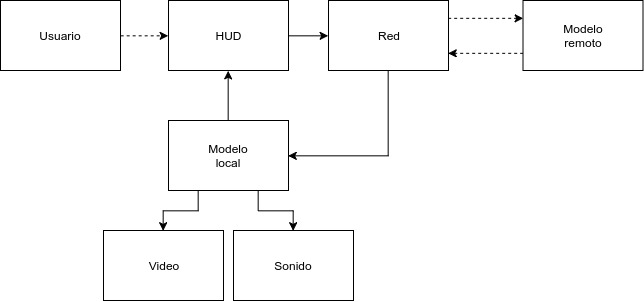
\includegraphics[width=16cm]{../imagenes/esquema-bloques-cliente.jpg}
	\caption{\label{fig:esquema-bloques-cliente} Esquema en bloques del funcionamiento general del cliente.}
\end{figure}

>>>>>>> 8cce5ac0bb1a3f067882a86c1d5b3a1d01c6e723
\subsection{Video}
El renderizado del juego se realizó utilizando la biblioteca SDL, la cual fue encapsulada en el paquete \textit{video}. El encapsulamiento realizado contempla principalmente el uso de RAII para la adquisición de recursos, tales como texturas o contextos de renderizado y el control de errores mediante excepciones.

Para maximizar el rendimiento del juego y minimizar el consumo de recursos se decidió utilizar únicamente texturas. Si bien esto es positivo desde el punto de vista del rendimiento, implicó una fuerte dependencia al contexto de renderizado ya que las texturas dependen directamente del mismo (a diferencia de las superficies, que se convierten al momento de renderizarlas).  

Esta fuerte dependencia genera dos grandes problemas:
\begin{itemize}
\item No se pueden conocer las dimensiones de las imágenes hasta el momento del primer renderizado.

Con lo cual, si se quisiera dimensionar dinámicamente un botón para un panel no podría hacerse en el constructor del mismo, sino que se debe posponer hasta el primer renderizado (a menos que se arrastre el contexto de renderizado por todos lados).

\item No se puede almacenar localmente la textura como caché.

Esto es debido a que si en el próximo renderizado se cambia de contexto entonces las texturas se invalidarían dado que fueron creadas para el primer contexto. Este caso podría suceder en el supuesto que se cambie de ventana, por ejemplo al pasar a pantalla completa.
\end{itemize}

El primer problema fue solucionado evitando el uso de dimensionado dinámico. En la mayoría de los casos esto no es necesario, y en los pocos casos donde sería útil se pudo reemplazar con tamaños de boton fijos.

El segundo problema es un poco más complicado y casi obligatorio de resolver debido a que el rendimiento del cliente depende mucho del almacenamiento de texturas prerenderizadas en caché. Para solucionarlo se creó una clase \textit{AdministradorTexturas} que se encarga de crear texturas y sus derivados (cargar imágenes, renderizar texto) y además proveer un almacenamiento de tipo ID->Textura de modo de poder almacenar las texturas directamente en el contexto de renderizado. Esto permite que cada entidad que requiera almacenar una textura en caché pueda tener un identificador de la misma y preguntarle al contexto de renderizado si ``la textura ya fue renderizada en ese contexto''. En el caso de que cambiara el contexto simplemente se renderiza nuevamente y se almacena en el contexto nuevo.

En gran parte estos problemas se deben a considerar que la ventana no debería ser un Singleton ni ningún tipo de variable de acceso global. Para poder cargar un sprite es necesario tener la ventana, ya que la carga de texturas está ligada directamente al contexto de renderizado a utilizar. Esto no es un problema si sólo se quiere renderizar el sprite en la pantalla, pero, si se quiere realizar acciones basándose en las \textit{dimensiones} de este sprite, entonces es necesario tener el contexto de renderizado para poder cargarlo y luego obtener sus dimensiones.

Este problema no es tan importante para renderizar el terreno de juego y sus unidades pero sí representa un problema grave al renderizar el HUD. El HUD en particular requiere conocer los tamaños de los botones, que en muchos casos están ligados al tamaño de los sprites y esto es escencialmente necesario para poder posicionarlos en la ventana. Gran parte del posicionamiento de sprites se realiza en los constructores de los widgets; los cuales, en el caso de los botones no tendrían tamaño hasta no ser renderizados al menos una vez (de modo de obtener el contexto de renderizado y las dimensiones del mismo). Lo mismo sucede para los widgets que contienen texto; no se puede dimensionar el texto hasta no pasar por el contexto de renderizado.

Como un \textit{workaround} para este problema se fijaron los tamaños de distintos widgets a constantes fijas. Esto solucionó a priori el problema pero le da una rigidez al HUD que termina siendo negativo contra la flexibilidad que ofrecen los widgets.

La ventana está modelada mediante widgets lo cual permite organizar los elementos de una forma jerárquica relativamente sencilla. El renderizado de la misma arranca en el widget raíz y luego va hacia abajo por la jerarquía dibujando cada widget según corresponda. 

Este modelo jerárquico resolvió casi todos los problemas, menos uno: gráficos que se superponen sobre lo dibujado, en particular los mensajes de información sobre los botones de construcción (\textit{tooltips}). Si bien para todos los elementos que se ubican en la ventana de forma \textit{relativa} el modelo funcionó correctamente, para los elementos con posicionamiento \textit{absoluto}, como es el caso particular de los \textit{tooltips} este modelo no sirve. 

Para resolver este problema se le agregó a la ventana un nuevo plano. La ventana así se compone de dos planos: un plano trasero, o \textit{plano relativo} y un plano frontal o \textit{plano absoluto}. El plano relativo es donde se dibujan todos los widgets y todos los elementos que pueden ubicarse mediante el posicionamiento relativo de elementos; en este plano sucede la mayor parte del renderizado. Por otra parte el plano absoluto es donde se dibujan los elementos que requieren un posicionamiento más libre.
Los nombres trasero y frontal se deben a que el plano frontal se dibuja por encima del plano trasero.

El área de juego es un widget más que se encarga de procesar los eventos de mouse y teclado que se corresponden con acciones en el juego, tales como seleccionar unidades, ubicar un edificio, etc. 
El renderizado de la misma es jerárquico también, pero no está basado en widgets. El terreno de juego, las unidades y edificios se renderizan de forma diferente ya que se posicionan de forma diferente.

El terreno de juego tiene un tamaño mucho mayor al tamaño de la ventana, ya que al tener dos jugadores o más lo normal es que aparezcan en zonas donde no se vea uno del otro. 

Para poder renderizar el fragmento que se está observando se utiliza una cámara que tiene como funcionalidad traducir las posiciones lógicas en visuales y viceversa. Sólo se renderiza en la ventana aquellas partes que están en el área de la cámara. 

<<<<<<< HEAD
=======
\begin{figure}[H]
	\centering
	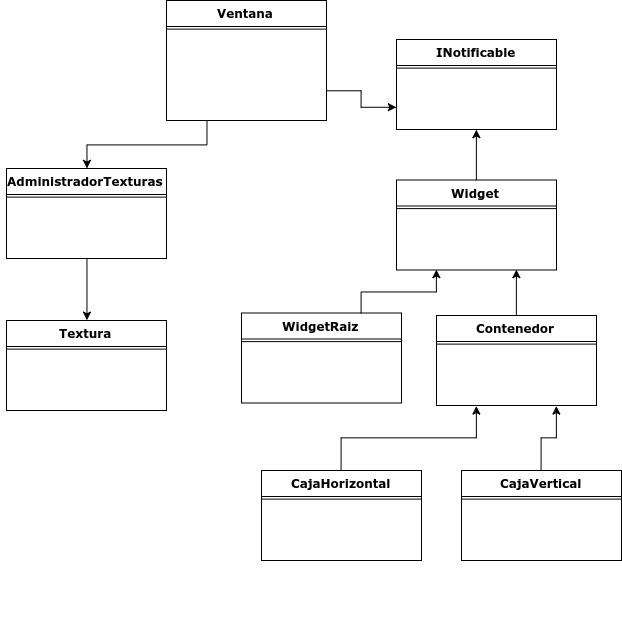
\includegraphics[width=12cm]{../imagenes/cliente-esquema-video.jpg}
	\caption{\label{fig:cliente-esquema-video} Esquema general del encapsulamiento de video.}
\end{figure}

>>>>>>> 8cce5ac0bb1a3f067882a86c1d5b3a1d01c6e723
\subsection{Sonido}
Para el sonido se decidió implementar un patrón de diseño Singleton. La razón para la elección del mismo es que díficilmente cambie el contexto de mezclado de sonidos a lo largo del juego (como sí podría pasar en el caso de un cambio de resolución con el video).

El subsistema de sonido es un encapsulamiento de SDL muy sencillo que se tiene tres funciones principales:
\begin{itemize}
\item Almacenar los sonidos y música en caché
\item Reproducir sonidos y evitar que se superpongan sonidos iguales
\item Reproducir música de fondo
\end{itemize}

En particular debe notarse que el sistema mismo evita reproducir dos sonidos iguales al mismo tiempo pero no evita la superposición de  sonidos distintos superpuestos (ya que perdería el sentido del mezclador).

\subsection{Red}
La comunicación a través de la red con el servidor se encapsuló en la clase Servidor. La misma tiene dos modos de operación: sincrónico y asincrónico. 

Toda la comunicación que se realiza desde el lanzador del juego se hace en modo sincrónico, ya que en este momento los tiempos de espera de la red no son problemáticos; la entrada de usuario suele ser lenta en general.

Por otra parte, toda la comunicación que se realiza durante el juego se hace de forma asincrónica. A medida que llegan los mensajes del servidor se van encolando hasta que el ciclo de juego decida procesarlos.

Tanto la comunicación sincrónica como la asincrónica se realizó utilizando el formato de serialización JSON ya que nos permitió depurar fácilmente el envío de mensajes. En caso de querer cambiarse, la serialización está encapsulada en la clase Conexión de modo que modificando los métodos enviar y recibir se puede optar por una serialización diferente.

Para notificar al modelo de los cambios remotos se utilizó un sistema de eventos serializables. La clase Servidor se encarga recibir los datos e ir almacenando los eventos en una cola. Cada evento irá modificando el modelo de juego según corresponda al momento de ser procesado.

\subsection{Lanzador}
El lanzador del modelo se desarrolló en Qt5, está compuesto de tres pantallas/estados que son: conexion, en lobby y en sala. 

El estado de conexión es el estado inicial y es el que permite conectarse a un servidor remoto. Una vez conectado se pasa al estado ``en lobby'', donde uno puede ver las salas disponibles, elegir una sala o crear una nueva.

Al ingresar a la sala se pasa a la etapa final. En esta última el jugador puede ver a el estado de sus compañeros de partida, elegir la casa con que va a jugar y lanzar el cliente.

Inicialmente el lanzador iba a soportar notificaciones push, de modo que en el momento en que el servidor detecte un evento se lo indique directamente sin que el mismo tenga que preguntar al servidor. Por problemas generales y falta de tiempo esta característica no se pudo implementar pero se la reemplazó solicitando actualizaciones al servidor cada un determinado período de tiempo, actualmente configurado en 10 segundos.

\subsection{Modelo}
El modelo de juego se compone de cinco entidades principales: Juego, Infraestructura, Ejercito, Terreno y HUD. 

Juego es el administrador general de la partida y se encarga principalmente de actualizar el estado general de la partida y de manejar las variables del jugador tales como la energía y el dinero disponible.

Infraestructura y Ejercito son los administradores de edificios y tropas, respectivamente. Los mismos se encargan de manejar las colas de construcción / entrenamiento, determinar a quién le pertenece un edificio o tropa y emitir los eventos sonoros correspondientes a bajas y ataques.

El Terreno es un componente central en el juego y particularmente en el cliente. El mismo permite resolver las solicitudes puntuales o de área del usuario, por ejemplo, en el caso en que el usuario arrastra un para generar un rectángulo en la ventana y seleccionar las tropas. A su vez el mismo resuelve otras solicitudes, por ejemplo si se puede construir un edificio en la posición indicada.

El HUD por otra parte es el punto de entrada a la visualización head-up. El mismo renderiza sobre la ventana los elementos extra tales como botones, el cursor del mouse, el rectángulo de selección, el dinero disponible, etc. A su vez actúa de controlador principal de la partida obteniendo la entrada del mouse y el teclado.

<<<<<<< HEAD
=======
\begin{figure}[H]
	\centering
	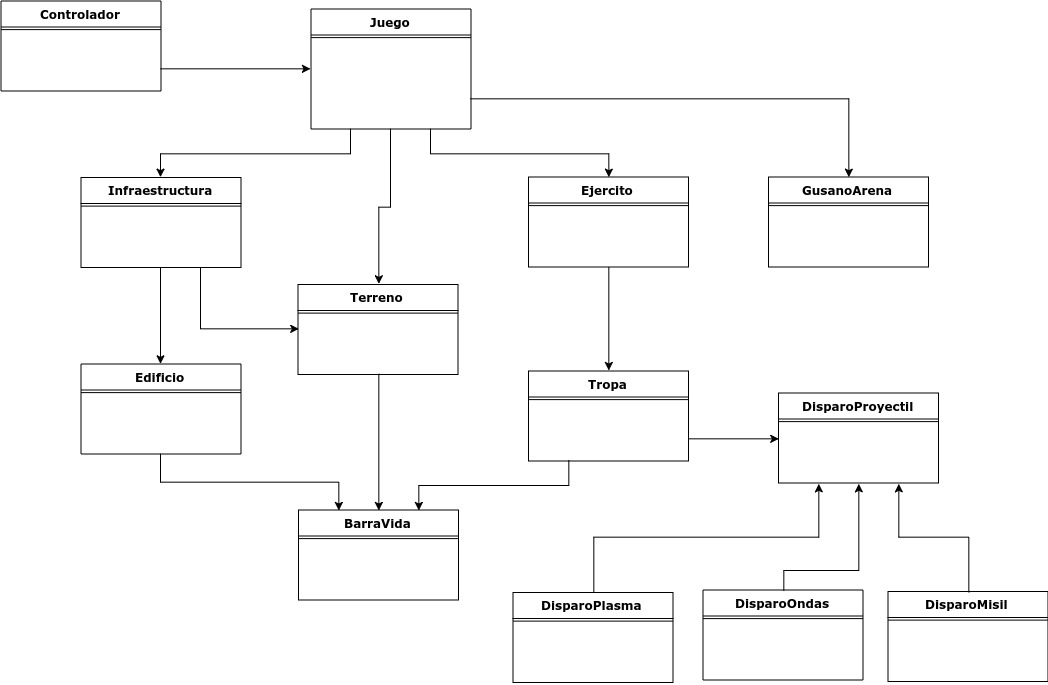
\includegraphics[width=14cm]{../imagenes/esquema-cliente-modelo.jpg}
	\caption{\label{fig:esquema-cliente-modelo} Esquema general del modelo local.}
\end{figure}

>>>>>>> 8cce5ac0bb1a3f067882a86c1d5b3a1d01c6e723
\subsubsection{Infraestructura y Ejército}
Para el modelo gráfico de tropas y edificios se decidió implementar un diseño basado en prototipos. El mismo nos permitió tener menos clases, evitar la herencia y además tener más flexibilidad a la hora de ultimar detalles cómo el posicionamiento de los sprites, ya que tomamos la decisión de bajar esta información a archivos de datos. Tanto las tropas como los edificios cargan su modelo de datos desde archivos en formato JSON.

\subsubsection{Visualización Head-Up}
Para la implementación del HUD se decidió utilizar un diseño basado en Widgets. Este diseño si bien no es sencillo de implementar, una vez resuelto permitió tener un sistema de eventos mucho más sencillo, mucha más movilidad a la hora de diseñar el HUD en sí y simplificar el problema de las dimensiones variables de la ventana. Con el diseño basado en Widgets, al correr el cliente en modo ventana o en modo pantalla completa el mismo se ajusta automáticamente según el espacio disponible.

La implementación de eventos en los widgets se hizo de forma directa utilizando herencia.

El componente central del HUD es el área de juego. La misma se encarga de renderizar el modelo y responder a la interacción del usuario, ya sea desde el mouse o el teclado. Estas interacciones pueden ser desde un movimiento de cámara hasta solicitar un ataque.

<<<<<<< HEAD
=======
\begin{figure}[H]
	\centering
	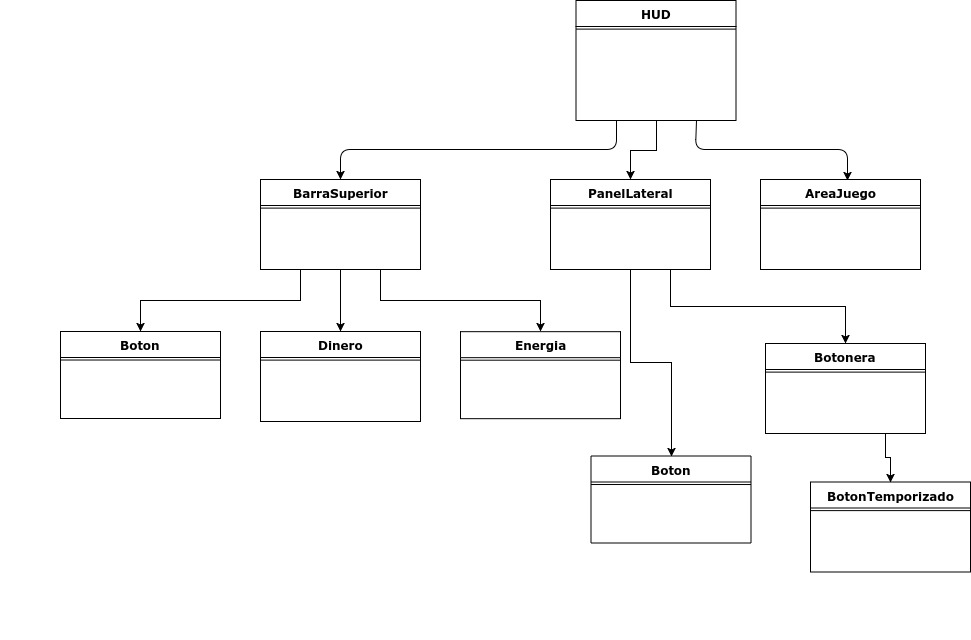
\includegraphics[width=14cm]{../imagenes/cliente-esquema-HUD.jpg}
	\caption{\label{fig:cliente-esquema-HUD} Esquema general del HUD.}
\end{figure}

>>>>>>> 8cce5ac0bb1a3f067882a86c1d5b3a1d01c6e723
\subsection{Ciclo de juego}
El ciclo de juego en el cliente se realiza de la siguiente manera:
\begin{enumerate}
    \item Renderizar el juego
    \item Procesar eventos locales (mouse y teclado)
    \item Procesar eventos remotos (servidor)
    \item Avanzar el juego en un fragmento de tiempo
\end{enumerate}

\subsubsection{Renderizar el juego}
En este punto simplemente se renderizan todos los elementos en la ventana. No se realiza ninguna modificación al juego, sólo se observa y renderiza.

\subsubsection{Procesar eventos locales}
En esta etapa se detectan y hacen derivan los eventos provenientes de la entrada del usuario tales como movimiento/click del mouse, teclado, cerrar la ventana, etc.

Al recibirse estos eventos se los envía al widget raíz que es el encargado de propagarlos hacia abajo hasta que algún widget decida procesar el evento.

En este punto el sistema de widgets agrega una optimización ``gratuita''. Debido a que la ventana se compone a partir de contenedores con posicionamiento horizontal y contenedores con posicionamiento vertical, los mismos actúan como una especie de árbol reduciendo la cantidad de widgets que deben ser procesados para indicar quién recibe un evento de mouse. 
Un contenedor con posicionamiento horizontal particiona el espacio según la coordenada X, mientras que un contenedor con posicionamiento vertical lo hace sobre la coordenada Y. Si bien no es una gran optimización, en grandes jerarquías esto evita revisar todos los widgets creados.

Es en este momento que se realiza la comunicación con el servidor para indicar las intenciones del usuario. El HUD es el encargado de detectar estas intenciones y luego comunicarselas al servidor.

\subsubsection{Procesar eventos remotos}
Luego de haberse procesado los eventos locales se procesan todos los eventos que el servidor haya comunicado. En este momento se actualiza el modelo de juego de modo de sincronizar las posiciones de tropas, crear o destruir nuevos edificios, alterar los valores de dinero / energía y demás.

Para esto se diseñaron distintas clases de eventos cuya responsabilidad es actualizar los distintos fragmentos del modelo según corresponda.

\subsubsection{Avanzar el juego en un fragmento de tiempo}
Una vez que se procesaron todos los eventos, se realiza la actualización temporal del modelo. Esta actualización es la que se encarga de interpolar el movimiento de tropas, cambiar el estado de los botones temporzados, animar la construcción y destrucción de edificios y cualquier otra acción que dependa del tiempo.

\newpage
\section{Servidor}

\subsection{Requerimientos de software}
Para compilar, desarrollar, probar y depurar el programa es necesario contar con un SO Linux, compilador GCC 7.3.0, biblioteca Json para c++ modernos y cmake.

\subsection{Descripción general}
El servidor modela a los clientes con dos hilos y una cola: un hilo y una cola para enviar los mensajes, y un hilo y callbacks para recibir los mensajes. 

Para el envío de mensajes se utiliza una cola para poder ofrecer al modelo de juego una latencia mínima. Esto permite que si un cliente por algún motivo es lento para recibir, el mismo quede esperando en un hilo separado hasta que la red se descongestione y el modelo pueda seguir con su procesamiento. 

Para la recepción de mensajes se decidió utilizar callbacks debido a su simplicidad. Utilizar una cola por cliente para recibir los mensajes implicaría distintos problemas, tales como necesitar tener un hilo específico para poder reunir los mensajes de todos los clientes y comunicarselos al modelo o tener que pasar una cola a todos los clientes.  
Dado que el servidor trabaja en dos etapas: etapa de sala/lobby y etapa de partida, la solución más sencilla consistió en tener un callback en cada cliente que indique que se recibieron nuevos datos. De este modo se configura el callback en la etapa de lobby para que procese los mensajes del lobby y luego se configura un callback en la partida que simplemente encole el mensaje en la cola de mensajes 
del modelo.

Esto nos permitió tener sólo dos hilos por cliente y un hilo por partida, de modo que, en el caso general la cantidad de hilos corriendo en el servidor está dada por la siguiente expresión:
$$ n_{hilos} = 2 + 2 \cdot n_{clientes} + n_{partidas_activas}$$

Es decir, el hilo principal, el hilo que acepta conexiones, dos hilos por cliente y un hilo por partida activa.
La etapa de lobby/sala no requiere hilos ya que se aprovechan los hilos de recepción de los clientes.

Para toda la comunicación cliente-servidor se utilizó el formato JSON. La elección del mismo es que es un formato ampliamente conocido, sencillo de usar, y por sobre todas las cosas, al serializarse como texto plano simplificó mucho la depuración de problemas de conexión.

\subsubsection{Interacción con el modelo de juego}
Para poder disociar el servidor y todo lo que implique conectividad y concurrencia del modelo de juego, se diseñaron dos interfaces: \texttt{IModelo} e \texttt{IJugador}.

La primera es la interfaz que el servidor espera encontrar y que el modelo de juego debe implementar. La misma consiste en unos pocos métodos que permiten interactuar con el servidor, como iniciar la partida o saber si terminó; y métodos que significan mensajes provenientes desde un jugador. El modelo de juego sólo debe implementar estos métodos para poder escuchar a los jugadores y puede asegurarse de que los métodos se ejecutarán de forma sincrónica, protegidos por el servidor.

La segunda es la interfaz que el modelo espera encontrar y que el servidor debe implementar. Esta permite que el modelo le \textit{hable} a los jugadores y se compone principalmente de todos los mensajes que el modelo le puede enviar a un determinado jugador, más un par de métodos misceláneos que permiten conocer el nombre del jugador, la casa a la que pertenece o un ID numérico.
\subsection{Modelo}
A la hora de diseñarlo siempre se tuvo en mente la versatilidad del modelo, de forma tal que el modelo no limite las capacidades del juego, sino que por lo contrario ayude y sea transparente a la hora de querer modificar/agregar funcionalidades.
Para ello se trato de dividir las responsabilidades correctamente encampuslando la informacion necesaria de forma tal que el codigo quede lo mas desacoplado posible.\\
Para el modelado del juego se usaron varios patrones de diseño entre los que se destacan, Type Object y Prototype.\\
El primero fue de gran ayuda a la hora de incorporar la información sobre las tropas y edificios desde archivos externos. Haciendo uso de este patron tenemos clases, por ejemplo, "Edificio" que tiene como atributo "EdificioBase", esta ultima es la que encapsula y carga los datos correspondientes desde los archivos externos.\\
Al hacer uso del patron Prototype junto a Type Object pudimos lograr que las clases "bases" o "genericas" solo se creen una vez. Esa única instancia se almacenan en clases cuyas responsabilidad es crear nuevas instancias a partir de los prototipos originales, es decir, las instancias guardadas saben como "clonarse" y almacenan la informacion común a todas las instancias. 

\subsection{Clases, interfaces y estructuras}

A continuación describiremos en profundidad las clases, las interfaces y las estructuras utilizadas por el Servidor.

\begin{itemize}

\item main: delega el procesamiento del archivo de configuración en la clase ProcesadorConfiguración y si no hubo errores durante el procesamiento instancia un objeto de la clase Servidor con dicha configuración como argumento. Lanza un std::thread que ejecuta el método correr de la clase Servidor.

\item ProcesadorConfiguracion: se encarga de almacenar la configuración del servidor en memoria. Procesa el puerto en el que el servidor \textit{escucha}  conexiones nuevas, la información de las tropas y los edificios y los mapas cargados.

\item SocketAceptador: es una encapsulación RAII de un socket bloqueante utilizado por Servidor para aceptar conexiones con clientes nuevos.

\item Servidor: dentro de la clase Servidor, el método correr es prácticamente un ciclo while en el que el socket aceptador acepta conexiones con nuevos clientes, una vez concretada dicha conexión se agrega e inicializa un objeto Cliente cuyo constructor tiene como parámetro el socket conexión asociado al cliente (el socket que es devuelto por el accept del socket aceptador del servidor). También se agrega el nuevo cliente al Lobby. El ciclo puede ser detenido desde el main por el usuario mediante el método de centinela.

\item Cliente:

\item Sala:
\item Cliente: Encapsula la conexión del cliente y los hilos de transmisión y recepción.

\item Sala: Gestiona el modelo de juego para una partida y los jugadores que están conectados a la misma.

\item Lobby: el lobby es el lugar en el que están los clientes que se conectaron al Servidor pero todavía no se unieron a ninguna Sala. Recibe en el constructor la data de la configuración (mapas, edificios y ejércitos) ya que desde esta clase se crean las Salas (completar).

\item AdminMapas: almacena los mapas JSON en un std::unordered\_map siendo las claves los nombres de los mapas y los valores los mapas, siendo estos de tipo nlohmann::json. Tiene implementadas funcionalidades como obtener un mapa por su nombre, saber si existe un mapa con un determinado nombre y saber la cantidad de jugadores que tiene un determinado mapa.

\item IModelo: es la interfaz que el servidor espera encontrar y que el modelo de juego debe implementar. La misma consiste en unos pocos métodos que permiten interactuar con el servidor, como iniciar la partida o saber si terminó; y métodos que significan mensajes provenientes desde un jugador. El modelo de juego sólo debe implementar estos métodos para poder escuchar a los jugadores y puede asegurarse de que los métodos se ejecutarán de forma sincrónica, protegidos por el servidor.

\item IJugador: es la interfaz que el modelo espera encontrar y que el servidor debe implementar. Esta permite que el modelo le \textit{hable} a los jugadores y se compone principalmente de todos los mensajes que el modelo le puede enviar a un determinado jugador, más un par de métodos misceláneos que permiten conocer el nombre del jugador, la casa a la que pertenece o un ID numérico.

\item ConexionJugador: es la clase que implementa la interfaz IJugador. Lo notifica a Cliente sobre las modificaciones en el modelo para que dicha clase se la envíe a los jugadores.

\end{itemize}

\subsection{Diagramas UML}
\begin{itemize}

\item Modelo del juego\\

En el siguiente diagrama de clases intenta dar una idea general de las relaciones entre clases y como se comunican para llevar a cabo las operaciones basicas dentro del juego.\\

\begin{figure}[H]
	\centering
	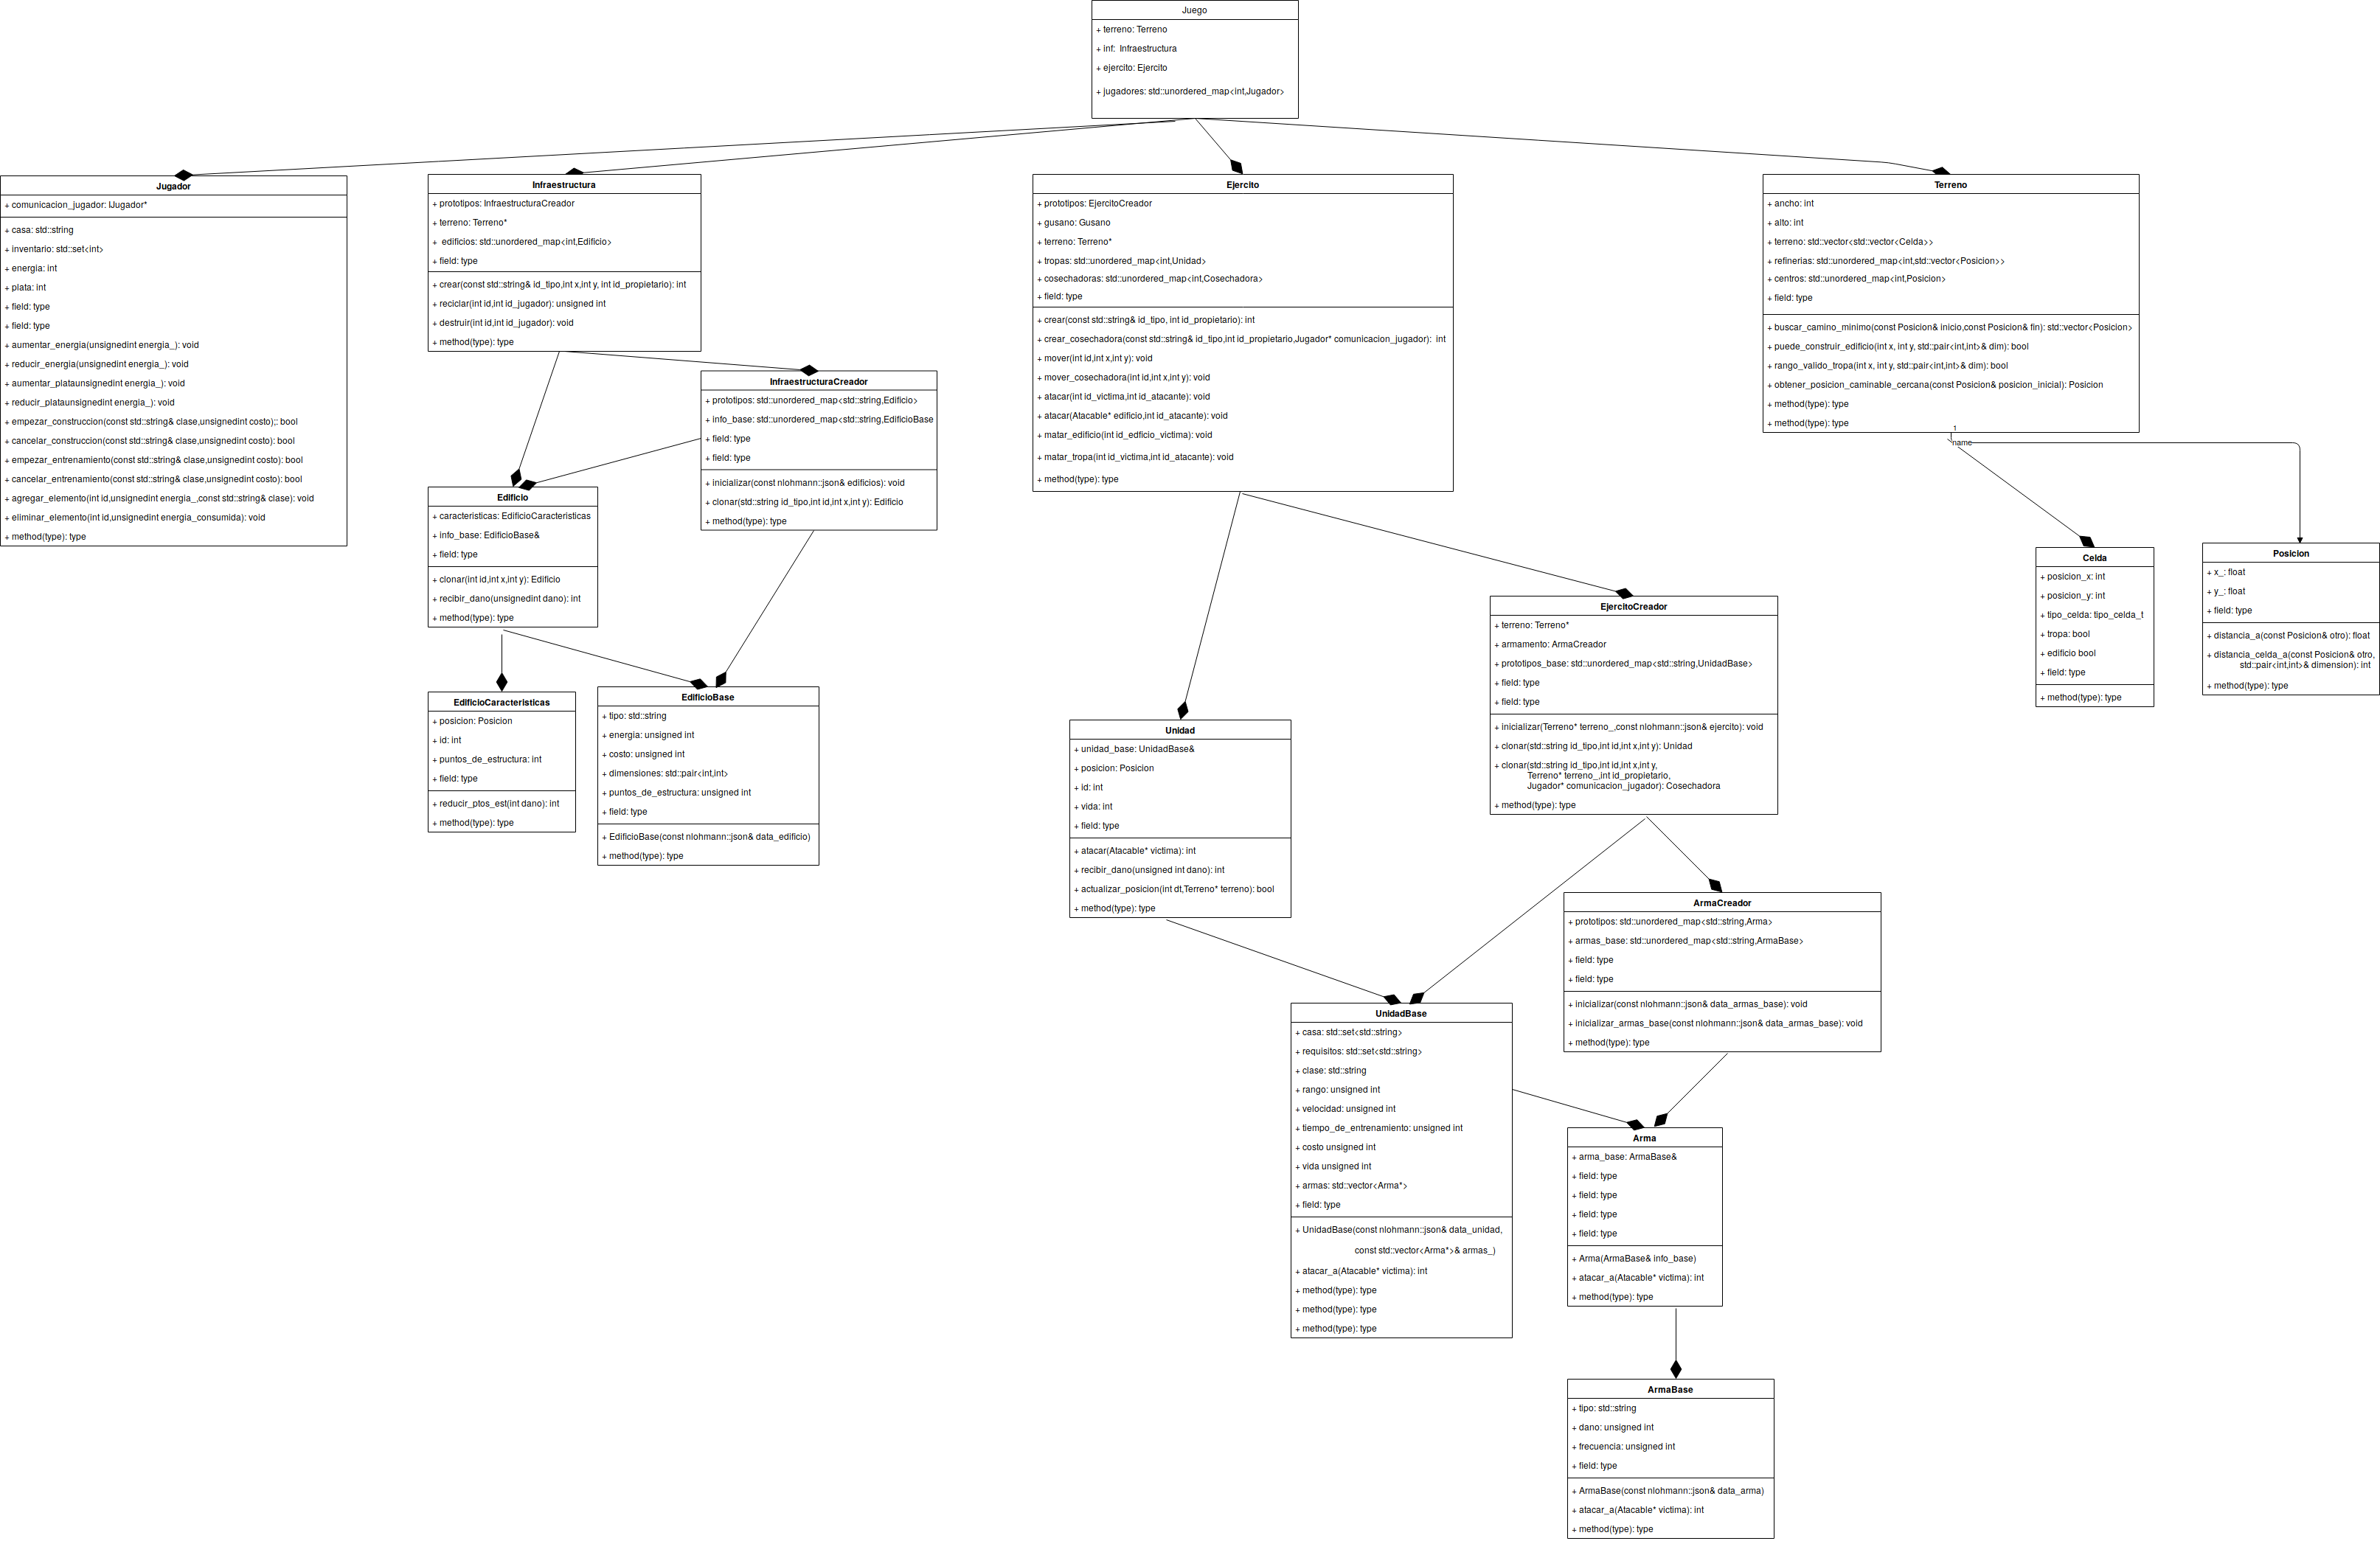
\includegraphics[width=0.8\textwidth]{../imagenes/modelo_clases.png}
	\caption{\label{fig:seq_uml_agregar_terreno} Diagrama de clases UML: modelo.}
\end{figure}

\item Secuencia de ataque\\
En el siguiente diagrama de secuencia se muestra como se realiza un ataque dentro del modelo, queda claro como se hace uso de polimorfismo y como se van delegando las tareas hasta llegar a la clase correspondiente.\\
\begin{figure}[H]
	\centering
	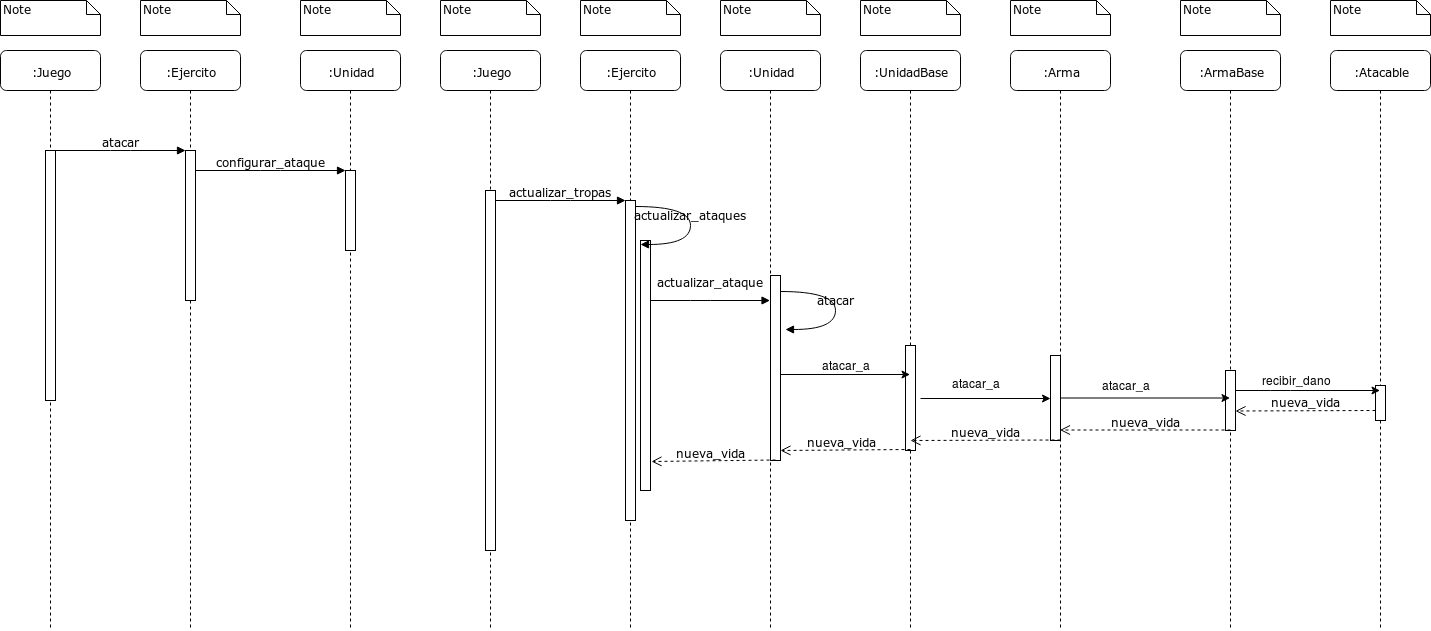
\includegraphics[width=0.8\textwidth]{../imagenes/secuencia_ataque.png}
	\caption{\label{fig:seq_uml_agregar_terreno} Diagrama de secuencia UML: atacar.}
\end{figure}

\end{itemize}

\subsection{Formato de los archivos de configuración}

Todos los archivos de configuración deben estar en formato JSON. A continuación se describe el contenido de los mismos

\begin{itemize}

\item Configuración general\\

El archivo de configuración general es un JSON que almacena el puerto de conexión del servidor, la ruta al archivo de datos de los edificios, la ruta al archivo de datos de los ejercitos y un array de rutas a los mapas disponibles.

\item Edificios\\

El archivo de edificios contiene la información relativa a los edificios que se pueden construir en el juego, sus imágenes y metadatos. Este archivo contiene un arreglo de objetos siendo cada objeto un nuevo tipo de edificio. Cada edificio tiene los siguientes datos: 

\begin{itemize}

\item ID:  este es el identificador del *tipo* de edificio. Debe ser único por cada clase de edificio distinto.

\item Nombre: el nombre *legible por humanos* del edificio, para mostrar en la interfaz gráfica.

\item ID:  este es el identificador del \textit{tipo} de edificio. Debe ser único por cada clase de edificio distinto.

\item Nombre: el nombre \textit{legible por humanos} del edificio, para mostrar en la interfaz gráfica.

\item Descripción: descripción del edificio para mostrar en la interfaz gráfica. No debe superar los 100 caracteres.

\item Metadata: metadatos del edificio, este campo sólo se utiliza para mostrar información extra al usuario (no afecta al juego). El mismo debe ser un objeto JSON donde la clave es un nombre de atributo y el valor debe ser el valor del mismo.

\item Energía: energía requerida por el edificio.

\item Costo: dinero requerido para construir el edificio.

\item Dimensiones: dimensiones, en celdas, del edificio.

\item Tiempo de construcción: tiempo, en segundos, requeridos para construir el edificio a velocidad normal.

\item Puntos de estructura: puntos de estructura (vida máxima) del edificio.

\item Capacidad de almacenamiento de especia: si el edificio puede almacenar especia, debe indicarse la cantidad en este campo.

\item Sprite base, construido y destruido : estos sprites definen cómo se dibujará el edificio en la pantalla de los clientes. El sprite *construido* representa el número de imagen a mostrar por el cliente cuando el edificio está construido y con más del 20\% de la vida. El sprite *destruido* representa el edificio cuando tiene menos del 20\% de la vida. El sprite *base* se utiliza cuando un edificio requiere componer su imagen a partir de dos sprites. Los parámetros `x` e `y` en los tres casos permiten desplazar el sprite para hacerlo coincidir con el sprite base.

\item Sprite base, construido y destruido : estos sprites definen cómo se dibujará el edificio en la pantalla de los clientes. El sprite \textit{construido} representa el número de imagen a mostrar por el cliente cuando el edificio está construido y con más del 20\% de la vida. El sprite \textit{destruido} representa el edificio cuando tiene menos del 20\% de la vida. El sprite \textit{base} se utiliza cuando un edificio requiere componer su imagen a partir de dos sprites. Los parámetros `x` e `y` en los tres casos permiten desplazar el sprite para hacerlo coincidir con el sprite base.

\item Sprite del botón de construcción: indica cual es el número de imagen correspondiente al botón de construir.

\end{itemize}

\item Ejércitos\\

<<<<<<< HEAD
El archivo de ejércitos es el que contiene toda la información requerida por el servidor y los clientes sobre los distintos tipos de tropa. El mismo debe estar en formato JSON y contener, **únicamente** un objeto con 
=======
El archivo de ejércitos es el que contiene toda la información requerida por el servidor y los clientes sobre los distintos tipos de tropa. El mismo debe estar en formato JSON y contener, \textbf{únicamente} un objeto con 
>>>>>>> 8cce5ac0bb1a3f067882a86c1d5b3a1d01c6e723
dos atributos: `armas` y `unidades`.  El atributo `armas` debe ser un arreglo de objetos con los siguientes atributos:


\begin{itemize}

<<<<<<< HEAD
\item ID: este es el identificador del *tipo* de arma. Debe ser único por cada clase de arma distinta. Este parámetro es obligatorio.
=======
\item ID: este es el identificador del \textit{tipo} de arma. Debe ser único por cada clase de arma distinta. Este parámetro es obligatorio.
>>>>>>> 8cce5ac0bb1a3f067882a86c1d5b3a1d01c6e723

\item Daño: el daño que hace el arma cada vez que es disparada.


\item Frecuencia de disparo: cuántas veces por segundo se debe disparar el arma.

\item Bonificaciones por clase de tropa: debe ser un objeto donde cada atributo es el ID de una tropa definida en `unidades` y el valor es el daño extra a realizar (daño total = daño + bonificación).

\item Bonificaciones por tipo de tropa: debe ser un objeto donde cada atributo es `vehiculo` o `unidad` para determinar si la bonificación aplica a vehículos o a unidades, respectivamente; y el valor el mismo es el daño extra a realizar.

\item Bonificaciones a edificios: indica el daño extra realizado por la tropa a los edificios.

\end{itemize}

El atributo `unidades` debe ser un arreglo de objetos con los siguientes atributos:  

\begin{itemize}

<<<<<<< HEAD
\item ID: este es el identificador del *tipo* de tropa. Debe ser único por cada clase de tropa distinta.

\item Nombre: el nombre *legible por humanos* de la tropa, para mostrar en la interfaz gráfica.
=======
\item ID: este es el identificador del \textit{tipo} de tropa. Debe ser único por cada clase de tropa distinta.

\item Nombre: el nombre \textit{legible por humanos} de la tropa, para mostrar en la interfaz gráfica.
>>>>>>> 8cce5ac0bb1a3f067882a86c1d5b3a1d01c6e723

\item Descripción: descripción de la tropa para mostrar en la interfaz gráfica. No debe superar los 100 caracteres.

\item Metadata: metadatos de la tropa, este campo sólo se utiliza para mostrar información extra al usuario (no afecta al juego). El mismo debe ser un objeto JSON donde la clave es un nombre de atributo y el valor debe ser el valor del mismo. Un ejemplo de esto sería lo siguiente: `\{"Rango": "3 casillas"\}`.

\item Casa: identificadores de las casas que pueden construir este tipo de edificio. Debe ser un arreglo que contenga al menos una y como máximo tres de las mencionadas en el valor por defecto. 

\item Requerimiento: indica qué edificios son requeridos para poder entrenar este tipo de tropa. Observar que los ID son strings que deben coincidir con los IDs definidos en el archivo de edificios.

\item Armas: arreglo con los ID de armas que posee la tropa. El ID debe coincidir con el indicado en el atributo `armas` de este mismo archivo.

\item Rango: rango de ataque de la tropa, en casillas.

\item Velocidad: velocidad de la tropa, en km/h.

\item Tiempo de entrenamiento: tiempo de entrenamiento de la tropa en minutos. Observar que el valor es número de punto flotante.

\item Costo: dinero requerido para entrenar la tropa.

\item Vida: vida máxima de la tropa.

\item Sprite base, techo y disparo: estos sprites definen cómo se dibujará la tropa en los clientes.  Sprite base define el primer sprite de una secuencia de sprites. Para el caso de los vehículos, este sprite define el primero de los 32 sprites de orientación del vehículo. Para el caso de las unidades, este sprite define el primero de las animaciones de caminar, disparar y fallecer.  Sprite techo sólo se utiliza en el caso de los vehículos y define el primero de 32 sprites orientables que se dibujará sobre el techo del sprite base.

\item Sprite de descarga: para las unidades que recolectan especia, este sprite indica cual es el primero de la animación de descarga de la especia en las refinerías.

\item Sprite del botón de entrenamiento: indica cual es el número de imagen correspondiente al botón de entrenar.

\item Tipo de unidad: indica si es una unidad o un vehículo. Los valores admitidos son `unidad` y `vehículo`.

\end{itemize}

\end{itemize}

<<<<<<< HEAD
=======

>>>>>>> 8cce5ac0bb1a3f067882a86c1d5b3a1d01c6e723
\newpage
\section{Editor}

\subsection{Requerimientos de software}
Para compilar, desarrollar, probar y depurar el programa es necesario contar con un SO Linux, compilador GCC 7.3.0, Qt 5, QtDesigner, User Interface Compiler (uic), biblioteca Json para c++ modernos y cmake.

\subsection{Descripción general}

El Editor fue codeado en el lenguaje C++ y además se utilizó la librería gráfica Qt 5 y la librería JSON para C++ modernos . La aplicación esta compuesta por 2 elementos principales: el dialogo de bienvenida y el editor de mapas. El dialogo de bienvenida contiene 2 botones que permiten elegir entre crear un mapa desde cero y cargar un mapa creando anteriormente. Luego de configurar el nuevo mapa o de elegir el mapa ya creado con anterioridad se abre la ventana del editor de mapas. Dicho editor esta compuesto por 3 elementos: el terreno del mapa, la pestaña que contiene los distintos terrenos ubicables en el mapa y la barra con el menu.\\

Se utilizo Qt 5 para diseñar la interfaz gráfica y para atrapar los eventos que el usuario genere al utilizar dicha interfaz gráfica. Para almacenar un mapa utilizamos el formato JSON al ser un formato ampliamente conocido y sencillo de usar.

\subsection{Clases, interfaces y estructuras}

A continuación describiremos en profundidad las clases, las interfaces y las estructuras utilizadas por el Editor.

\begin{itemize}

\item main: función de entrada de la aplicación. Muestra el dialogo de bienvenida e inicializa el loop de la ui.

\item DialogoBienvenida: clase que hereda de QDialog, por lo tanto representa a una ventana de diálogo. Contiene 2 QPushButton, uno para crear un mapa y el otro para cargar un mapa. Como layout utiliza un QFormLayout aunque podrían usar otros sin cambiar la funcionalidad. Los eventos de click de los botones generan la ejecución de los métodos DialogoBienvenida::mostrar\_dialogo\_crear\_mapa y DialogoBienvenida::mostrar\_dialogo\_cargar\_mapa. El primer método muestra otro diálogo conformado por QSpinBox para poder elegir la cantidad de jugadores y el tamaño del mapa y el segundo muestra un QFileDialog para elegir el archivo del mapa guardado. Al final de ambos métodos se iniciliza el objeto Editor.

\item Editor: clase que hereda de QMainWindow ya que trae por defecto un QMenuBar, también implementa la interfaz 'Observador'. Se encarga de inicializar 'Mapa' y 'Tabs', de implementar respuestas a clicks en el QMenuBar (desde mostrar diálogos para modificar la configuración del mapa hasta guardar el mapa o cargar otro mapa) y oficia de intermediario entre el Mapa y la pestaña de Terrenos. Es observador de su propio 'Mapa' y se encarga de actualizar el terreno de un 'LabelMapa' en el caso de que este sea clickeado y a su vez este clickeado un 'LabelTab'. En el caso especial de que el LabelTab sea el de un jugador, se hacen verificaciones extras (por ejemplo este solo puede ubicarse sobre la roca) y estas verificaciones las delega en Mapa. 

\item Mapa: clase que implementa la interfaz 'ObservadorMapa' para justamente observar los 'LabelMapa' y ser notificado cuando uno de estos es clickeado. Se encarga de generar los 'LabelMapa' y agregarlos a un QGridLayout scrollable para representar un mapa. Tambien almacena las posiciones de los distintos jugadores ubicados por el usuario. El 'Editor' delega el cambio de tamaño del mapa en esta clase al justamente tener toda la información de los labels que conforman al mapa en ese momento. 

\item Tabs: clase que implementa la interfaz 'ObservadorTabs' para justamente observar los 'LabelTab' y ser notificado cuando uno de estos es clickeado. Tiene como atributos un std::map con los sprites que son mostrados en la pestaña de Terrenos y un 'Sprite' que representa al sprite del 'LabelTab' que fue clickeado (puede ser ninguno). Dicho Sprite es solicitado por 'Editor' cuando es clickeado un 'LabelMapa' para poder actualizar dicho LabelMapa.

\item LabelTab: clase que hereda de QLabel ya que permite settearle un QPixmap y además puede atrapar el evento de click del mouse. Es el objeto que aparece en la pestaña de Terrenos del editor de mapas. A su vez es observado por otro objeto que implementa la interfaz 'ObservadorTabs'. Dicho observador es notificado cuando se hace click sobre el label. El observador luego se encarga de almacenar cual LabelTab fue clickeado y si debe dibujarse un marco de clickeado o debe ser borrado su marco de clickeado (caso en el que el LabelTab había sido seleccionado anteriormente). Tiene la función de devolver su 'Sprite' correspondiente que luego es utilizado por otras clases para actualizar la imagen de un 'LabelMapa' al ser este clickeado.

\item LabelMapa: clase que hereda de QLabel (por las mismas razones que 'LabelTab') y ademas porque puede atrapar los eventos de enter y leave mouse (solamente se utiliza para mostrar un marco negro alrededor del label para mejorar la interfaz del usuario). Es el objeto que aparece en el mapa. A su vez es observado por otro objeto que implementa la interfaz 'ObservadorMapa'. Dicho observador es notificado cuando se hace click sobre el label. El observador luego se encarga de verificar si hay que actualizar el terreno que representa el LabelMapa.


\item GeneradorSprites: clase encargada de la generación de elementos 'Sprite'. El método público 'generar\_sprites\_posibles' es utilizado por la clase 'Mapa' antes de cargar un mapa, su función es generar todos los Sprites posibles que pueden ser ubicados en un mapa y así evitar la repetición de generación de un 'Sprite' en particular. Por ejemplo el Sprite arena es el mas utilizado en los mapas y en mapas grandes pueden haber cientos de Sprites arena, para no generar mas de 100 veces el mismo QPixmap, este método lo genera un única vez y devuelve un std::map con todos los sprites posibles. Luego se le pasa por parámetro el Sprite al constructor de 'LabelMapa'.\\

Otro método público llamado 'generar\_sprite\_inicial', similar al anterior y pensado de la misma manera, genera un 'Sprite' que es elegido por nosotros como inicial o por default para completar un 'Mapa' creado desde cero. Elegimos que dicho Sprite por default sea el de la arena.\\

Finalmente implementa otro método público llamado 'generar\_sprite', utilizado por 'LabelTab' para generar los 'Sprite' de cada terreno que luego es mostrado en 'Tab'. Recibe como parámetro el id, el tipo y el vector de posiciones de los tiles de 8x8 dentro del archivo de terrenos .bmp (que es el único atributo de esta clase, en forma de QPixmap).

\item ManejadorJson: clase cuya función única es generar el mapa en formato JSON. Recibe por parámetro el nombre del archivo a generar, el tamaño del mapa, la posición de los jugadores y la información de los terrenos que conforman al mapa. Le quita responsabilidades a la clase 'Mapa'.

\item Sprite: estructura que representa a un sprite. Esta compuesta por 3 elementos: un id de tipo string, un int que representa al tipo y un QPixmap que es la imagen en sí misma.

\item Observador: interfaz implementada por 'Editor'. Es utilizado por 'Mapa' para avisarle a 'Editor' cuando se hizo un click sobre un 'LabelMapa', el método virtual tiene como único parámetro el id de dicho 'LabelMapa'.

\item ObservadorMapa: interfaz implementada por 'Mapa'. Es utilizado por 'LabelMapa' para avisarle al observador que fue clickeado. El método virtual tiene como único parámetro el id de dicho 'LabelMapa'. 

\item ObservadorTabs: interfaz implementada por 'Tabs'. Es utilizado por 'LabelTab' para avisarle al observador que fue clickeado. El método virtual tiene como único parámetro el id de dicho 'LabelTab'. 

\end{itemize}

\subsection{Diagramas UML}

\begin{itemize}

\item Comunicación Editor-Mapa-Tabs\\

En el siguiente diagrama de secuencia se aprecia como funciona la comunicación entre los objetos Editor, Mapa y Tabs al agregar con éxito un terreno al mapa.\\

\begin{figure}[H]
	\centering
	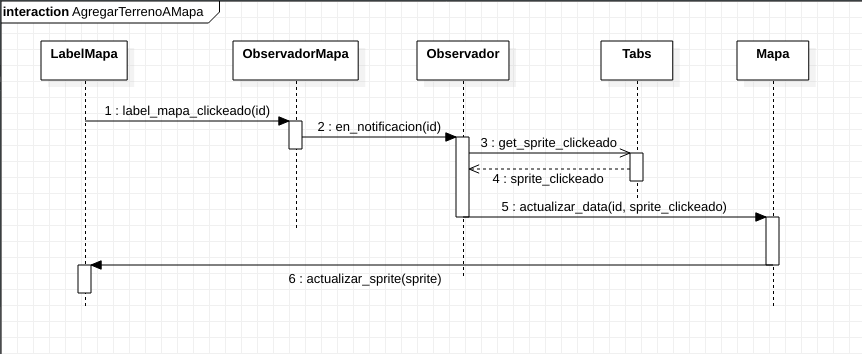
\includegraphics[width=0.8\textwidth]{../imagenes/seq_uml_agregar_terreno_editor.png}
	\caption{\label{fig:seq_uml_agregar_terreno} Diagrama de secuencia UML: agregar terreno al mapa.}
\end{figure}

\end{itemize}

\subsection{Descripción de archivos}

\begin{itemize}

\item Mapa\\

El Editor tiene la función de crear mapas y almacenarlos en memoria. Elegimos almacenarlos en el formato JSON por las razones indicadas en la 'Descripción general' del informe técnico en la sección del Editor. Dentro del archivo JSON se almacenas 2 arrays: uno representa la posicion de cada jugador en el mapa y el otro reprenta al mapa en si mismo. \\

El array de jugadores es de largo n siendo n la cantidad de jugadores. Cada elemento del array de jugadores a su vez es un array de largo 2 que representa la posición en el mapa del jugador, [X, Y]. \\

El array que representa al mapa también es una array de arrays. En este caso los arrays que se encuentran dentro del array principal son de largo k siendo k la cantidad de columnas del mapa y el array principal tiene un largo de h siendo h la cantidad de filas del mapa. Dentro de los arrays secundarios se ubican strings que representas los diferentes terrenos ubicables en el mapa. A continuación explicaremos que son esos strings en el item 'Sprites terrenos'.

\item Sprites terrenos\\

Los sprites de los terrenos están distribuidos en cuadrados de 8x8 pixeles en el archivo 'd2k\_BLOXBASE.bmp' cuyo tamaño es de 160x320 pixeles. A su vez cada tile del mapa tiene un tamaño de 32x32 pixeles, lo que serían 16 cuadrados de 8x8. A su vez cada tile tiene un id en formato string (por ejemplo: "arena1") y un tipo en formato int (por ejemplo: "0"). Para cada tipo de terreno existen distintos tiles con distintos ids (por ejemplo: "roca1", "roca2", étc.).\\

En el archivo terrenos.json se encuentran los distintos tipos de terrenos con sus respectivos tiles. Cada tile esta representado por un vector de ints de largo 16, cada elemento representa la posición de un cuadrado de 8x8 pixeles en el archivo .bmp indicado anteriormente, siendo el cuadrado que se encuentra en la esquina superior izquierda el 1, el cuadrado que se encuentra a su derecha el 2 y sigue contando de esa manera.

\item Editor.ui\\

Dicho archivo, editable con el programa Qt Designer, almacena la información de la interfaz gráfica (el diseño o wireframe, los distintos widgets, étc.).

\end{itemize}

\end{document}